% file: SVM_parallel_out.tex
%
% github        : ernestyalumni
% gmail         : ernestyalumni 
% linkedin      : ernestyalumni 
% wordpress.com : ernestyalumni
%
% This code is open-source, governed by the Creative Common license.  Use of this code is governed by the Caltech Honor Code: ``No member of the Caltech community shall take unfair advantage of any other member of the Caltech community.'' 

\documentclass[10pt]{amsart}
\pdfoutput=1
\usepackage{mathtools,amssymb,lipsum,caption}

\usepackage{graphicx}
\usepackage{hyperref}
\usepackage[utf8]{inputenc}
\usepackage{listings}
\usepackage[table]{xcolor}
\usepackage{pdfpages}
\usepackage{tikz}
\usetikzlibrary{matrix,arrows}

\usepackage{breqn} % for dmath


\usepackage{cancel} % for Feynman slash notation

\hypersetup{colorlinks=true,citecolor=[rgb]{0,0.4,0}}


%\oddsidemargin=15pt
%\evensidemargin=5pt
%\hoffset-45pt
%\voffset-55pt
%\topmargin=-4pt
%\headsep=5pt
%\textwidth=1120pt
%\textheight=595pt
%\paperwidth=1200pt
%\paperheight=700pt
%\footskip=40pt








\newtheorem{theorem}{Theorem}
\newtheorem{corollary}{Corollary}
%\newtheorem*{main}{Main Theorem}
\newtheorem{lemma}{Lemma}
\newtheorem{proposition}{Proposition}

\newtheorem{definition}{Definition}
\newtheorem{remark}{Remark}

\newenvironment{claim}[1]{\par\noindent\underline{Claim:}\space#1}{}
\newenvironment{claimproof}[1]{\par\noindent\underline{Proof:}\space#1}{\hfill $\blacksquare$}

%This defines a new command \questionhead which takes one argument and
%prints out Question #. with some space.
\newcommand{\questionhead}[1]
  {\bigskip\bigskip
   \noindent{\small\bf Question #1.}
   \bigskip}

\newcommand{\problemhead}[1]
  {
   \noindent{\small\bf Problem #1.}
   }

\newcommand{\exercisehead}[1]
  { \smallskip
   \noindent{\small\bf Exercise #1.}
  }

\newcommand{\solutionhead}[1]
  {
   \noindent{\small\bf Solution #1.}
   }


  \title[Support Vector Machines with constrained gradient descent]{Support Vector Machines (SVM) natively implemented in theano, entirely on the GPU with the CUDA backend, with constrained gradient descent}

\author{Ernest Yeung \href{mailto:ernestyalumni@gmail.com}{ernestyalumni@gmail.com}}
\date{29 mars 2017}
\keywords{Machine Learning, Support Vector Machines, Constrained Optimization, Projected Gradient Descent, CUDA C/C++, theano}

\begin{document}

\definecolor{darkgreen}{rgb}{0,0.4,0}
\lstset{language=Python,
 frame=bottomline,
 basicstyle=\scriptsize,
 identifierstyle=\color{blue},
 keywordstyle=\bfseries,
 commentstyle=\color{darkgreen},
 stringstyle=\color{red},
 }
%\lstlistoflistings

\maketitle

\tableofcontents

%\begin{multicols*}{2}


 











\begin{abstract}
\section{Executive Summary}

I implemented SVM natively in theano, and can run entirely on the GPU(s) (through the CUDA C/C++ backend).  Solving the \emph{constrained optimization} problem to train a SVM here used \emph{parallel reduce} algorithms; in fact a parallel reduce nested in side a parallel reduce.  The work complexity achieved in this case should be of $O(2\log{m})$ where $m$ is the total number of training examples, as opposed to $O(m^2)$ for Quadratic Programming (QP), such as Sequential Minimal Optimization (SMO).  Training on the same data set for vehicles as previous work for C/C++ library \verb|libsvm| that uses SMO, \verb|SVM_parallel| (what I call the described implementation here) achieves an accuracy of 95.1\% on test data, as opposed to 87.8\% for \verb|libsvm|.  What I'd like to do in the future is to train and test on larger datasets ($m>10000$) to test \verb|SVM_parallel| for its promising scalability, and to implement it as the outer layer of a deep neural network (DNN) for ``Deep SVM''.  

\end{abstract}



\section{Motivations and Introductions}\label{Sec:MotivationsIntroductions}

Support Vector Machines (SVM) can be used for (binary) classification in supervised learning on labeled data, being able to learn non-linear, higher-dimensional features and to predict a boundary line or discriminator between classes, through the so-called \emph{kernel trick}, which is really to presume a higher-dimensional Hilbert space to represent feature space $\mathcal{F}$ (i.e. $\mathcal{F}$ is a Hilbert space).

I considered the proposition of having, as a final, outer ``layer,'' of a deep neural network (DNN) to be a support vector machine.  Could it outperform the same DNN with a sigmoid or softmax function at the final layer?

To my knowledge, there was not a native implementation of SVM on theano, a Python framework for deep learning/DNNs.  Being that I sought to speed up learning/computation on the GPU(s) through the theano CUDA backend, it would seem to defeat the GPU speedup advantages if from the very last layer, a large global memory transfer had to occur from the GPU (with the last DNN layer), to a host CPU, \emph{serial}, implementation of SVM.  Global memory transfers are prohibitive expensive, for latency, i.e. time-wise, between host CPU and GPUs.\cite{CS344}    

The outline/plan/highlights for this (short) paper is as follows: in
\begin{itemize}
\item \ref{Sec:ConciseMathReview}, I review or summarize points in the theory for SVM, give derivations, etc., in which (this has all been done before; I sought to give a concise review)
  \begin{itemize}
\item \ref{SubSec:Hyperplanes}, I recap basic, elementary concepts motivating the linear discriminator concept and what hyperplanes are, and how they're defined by a \emph{linear} function
\item \ref{SubSec:MarginsLagrangian} - I continue to review and present derivations for the \emph{Lagrangian}, a Lagrange multiplier problem, we want to minimize, and apply the usual Karush-Kuhn-Tucker (KKT) condition to make progress in deriving the constrained optimization problem we seek to solve,
\item \ref{SubSec:Kerneltrick} kernel trick, with the feature space $\mathcal{F}$ as a Hilbert space, \ref{SubSec:slackvars} slack variables to deal with non-perfectly-separable data, and more derivation that was done before, but made explicitly here
\end{itemize}
\item \ref{Sec:DualFormulation}, the \emph{constrained optimization} problem we wish to solve for SVM
\item \ref{Sec:ConstrainedOptimization}, I translate how our constrained optimization problem is to be solved with \emph{projected gradient descent} or ``constrained gradient descent'' (as the projection operators enforce constraint equalities and inequalities).  As noted, this method/algorithm was chosen to utilize the (very useful) \verb|grad| method in the \verb|theano| software package.

  The Eqns. \ref{Eq:DualFormulationW}, \ref{Eq:ProjectionOpsAlgo} at the end of \ref{SubSec:ProjectedGradDescent} is the crux of the training method considered in this paper and code for SVM and was directly referred to when implemented in code.  
  \begin{itemize}
  \item I also show how to compute, in a numerically stable manner, the intercept $b$, after $\lambda_i$ Lagrange multipliers are found, and how to compute predictions $\widehat{y}$, in \ref{SubSec:binterceptcompute}, \ref{SubSec:Predictioncompute}
  \end{itemize}
  \item \ref{Sec:ConstrainedGradDescImplementation} the \emph{constrained gradient descent} to solve our constrained optimization problem is implemented and I detail its implementation using software package \verb|theano|, and especially its CUDA backend, so to run solely on the \emph{GPU}.  I give the rationale in deploying this constrained gradient descent as opposed to the Sequential Minimal Optimization (SMO) usually used in the predominant SVM software package (in C/C++) \verb|libsvm|.  Noteworthy, I also show that \textbf{work complexity goes from $O(m^2)$ to $O(2\log(m))$}.  
\item \ref{SubSec:Code} briefly tells where the code is made available and the 1-to-1 correspondence between the code and mathematical formulation.  I also note that \emph{novel use of theano's reduce within reduce}.  
\item \ref{SubSec:ResultsSampleDatasets} has \emph{results} that I try to compare with sample datasets used previously, that I've trained as quickly as possible.  Look here for the results; better yet, feel free to try the code and jupyter notebook and share benchmarks.\footnote{\href{https://github.com/ernestyalumni/MLgrabbag/blob/master/ML/SVM.py}{github:ernestyalumni/MLgrabbag/ML}, \href{https://github.com/ernestyalumni/MLgrabbag/blob/master/SVM_theano.ipynb}{github:ernestyalumni/MLgrabbag SVM theano.ipynb}}
\end{itemize}

\section{Concise Mathematical Review/Summary of the theory for SVM}\label{Sec:ConciseMathReview}

\subsection{Hyperplanes and distances to motivate the linear discriminator concept; Support Vector Machine name}\label{SubSec:Hyperplanes}

I'll recap basic, elementary concepts, from Clarke, Fokoue, and Zhang (2009) \cite{CFZ2009}, that motivate the concept of a linear discriminator classifying input data $X$.

Consider $\theta\in \mathbb{R}^d$, and a linear function $y$,
\begin{equation}\label{Eq:yforhyperplane}
\begin{aligned}
& y:\mathbb{R}^d \to \mathbb{R} \\
  & y(x) := \langle \theta,x \rangle +b 
  \end{aligned}
\end{equation}
Consider a ``level set'' at real number value $c\in \mathbb{R}$, $H_c(\theta,b)$:
\begin{equation}\label{Eq:H_cHyperplane}
H_c(\theta,b):=\lbrace x|y(x) = \langle \theta,x\rangle +b =c \rbrace 
  \end{equation}
where $\text{dim}H_c(\theta,b)=d-1$ is a \emph{hyperplane}.

$\theta\in \mathbb{R}^d$ is the normal vector to this hyperplane, since,
\[
\begin{gathered}
  \forall \, x^{(i)}, x^{(j)} \in H_c(\theta,b), \text{ then } \\
  \langle \theta, x^{(i)} \rangle + b = c = \langle \theta , x^{(j)}\rangle + b \Longrightarrow \langle \theta, x^{(i)} - x^{(j)} \rangle = 0 
  \end{gathered}
\]
and since $x^{(i)} - x^{(j)} \in TH_c(\theta,b)$, i.e. $x^{(i)} - x^{(j)}$ belongs in the tangent space to $H_c(\theta,b)$, $TH_c(\theta,b)$, then $\theta$, in general, is normal to the hyperplane ($\langle \theta, x^{(i)} - x^{(j)} \rangle =0$).

Given $z\in \mathbb{R}^d$, what is the distance from $z$ to this hyperplane $H_c(\theta,b)$, $d(z,H_c(\theta,b))$?  Consider $z* = z+t\theta\in H_c(\theta,b)$.  Then
\[
\begin{gathered}
  \langle \theta, z^*\rangle + b=c = \langle \theta,z \rangle + t\langle \theta, \theta\rangle + b = c \Longrightarrow t=\frac{ c-b-\langle \theta,z\rangle }{ \| \theta \|^2}  \\
  \text{ and so }
  d(z,H_c(\theta,b)) = \| t\theta \| = \frac{ | \langle \theta , z \rangle +b- c | }{\| \theta \| } 
  \end{gathered}
\]
Thus, for the perpendicular distance between 2 parallel hyperplanes, $H_c(\theta,b)$, $H_{c'}(\theta,b)$, can be found: choose a pt. from $H_c(\theta,b)$, without loss of generality, s.t. $z=\left( \frac{c-b}{\theta_1},0 , \dots 0 \right)$, so that
\[
\langle \theta,z \rangle + b=c \Longrightarrow \theta_1z^1 = c-b
\]
Then
\begin{equation}
d(H_c(\theta,b),H_{c'}(\theta,b)) = \frac{  | \langle \theta,z \rangle +b-c' | }{ \| \theta \| } = \frac{ | c-b+b-c' | }{ \| \theta \| } = \frac{ |c-c' | }{ \| \theta \| }
  \end{equation}

Given an input (data) domain $\mathcal{X}\subseteq \mathbb{R}^d$, for the case of binary classification, with total number of classes $K=2$, we can consider representing the outcomes $y$ for each input data example, $X \in \mathbb{R}^d$, in 2 ways:
\begin{equation}
  y\in \lbrace -1 , 1 \rbrace \text{ \textbf{or } } y\in \lbrace 0,1 \rbrace \text{ for } y \in \lbrace 0 , 1, \dots K-1\rbrace \, (K=2)
  \end{equation}
What ends up happening is that the distance between 2 hyperplanes, $c=-1,c'=1$ vs. $c=0,c'=1$, respectively, changes, as $d(H_c(\theta,b),H_{c'}(\theta,b)) = \frac{ |c-c' | }{ \| \theta \| }$, but its absolute value doesn't matter.  What matters is the form of $y:\mathbb{R}^d \to \mathbb{R}$, of Eq. \ref{Eq:yforhyperplane} which defines the hyperplane in Eq. \ref{Eq:H_cHyperplane}, notably in $\theta,b$.  The lesson is to \emph{be consistent with what the value of $y$ is to define what class $X$ belongs to}.  For instance, Bishop (2007) \cite{Bish2007} and Clarke, Fokoue, and Zhang (2009) \cite{CFZ2009} chooses to consider $y\in \lbrace - 1, 1 \rbrace, \, \forall \, X$ and I'll do the same here.

The name ``support vectors'' seems to come from this intuitive notion: $\theta \in \mathbb{R}^d$,$b$ are determined from $m$ input data examples $X^{(i)} \in \mathbb{R}^d$, $\forall \, i = 1, 2, \dots d$, and $\forall \, i$, the corresponding class label $y\in \mathbb{Z}$.  $\forall \, X^{(i)} \in \mathbb{R}^d$, imagine attaching normal vectors of the form $t\theta$, $t\in\mathbb{R}$ that extend out to the respective hyperplane, determined by $y^{(i)}$.  These imagined vectors ``support'' the respective hyperplane.  

An important takeaway is that the equation defining the hyperplane $H_c{(\theta,b)}$ in Eq. \ref{Eq:H_cHyperplane} is \emph{linear}.  

\subsection{Margins, cost functional or ``Lagrangian'', dual formulation}\label{SubSec:MarginsLagrangian}

With output, outcome $y\in \lbrace - 1, 1 \rbrace, \, \forall \, X$ input data example, the distance between the 2 hyperplanes, which are level sets of $c=-1,c'=1$, is
\[
\frac{2}{\| \theta \| }
\]
The method of SVM seeks to maximize this distance, also known as ``margin'', to make margins as big as possible.  

Clearly, this is equivalent to minimizing $\frac{1}{2} \| \theta \|^2$, with $\frac{1}{2}$ multiplication factor chosen, without loss of generality, to make taking derivatives of $\theta$ easier.

But we also have the following constraints.  We want to have a ``margin'' of $\frac{2}{\|\theta\|}$ between the hyperplanes that'll separate the input data examples $X^{(i)}$, $\forall \, i =1,2,\dots m$, for different classes, in this binary classification class, of those with $y^{(i)} \in \lbrace -1, 1\rbrace$, and so those $X^{(i)}$'s will ``fall far away'' from this ``margin'' and remain within its corresponding hyperplane $H_{c'=1}(\theta,b)$ or $H_{c=1}(\theta,b)$, thus defining these inequalities:
\begin{equation}\label{Eq:ineqconstraints}
  y^{(i)}(\langle \theta,x^{(i)} \rangle + b) - 1 \geq 0 \qquad\, \forall \, i = 1, \dots, m 
\end{equation}
So we want to find 
\[
\theta \in \mathbb{R}^d \backslash \lbrace 0 \rbrace ,\, b\in \mathbb{R}
\]
s.t.
\[
y^{(i)}(\langle \theta,x^{(i)} \rangle + b) - 1 \geq 0 \qquad\, \forall \, i = 1, \dots, m
\]
where $\frac{2}{\| \theta \|}$ is maximized, or equivalently, defining the so-called \emph{objective function} $f_{\theta}(\theta,b)$, minimize $f_{\theta}(\theta,b)$:
\begin{equation}
f_{\theta}(\theta,b) := \frac{1}{2} \| \theta \|^2 \qquad \, (\text{objective function})
\end{equation}

Consider then this cost functional, also known as the ``Lagrangian'', which we want to \emph{minimize}.  
\begin{equation}\label{Eq:costLagrangianL}
  \mathcal{L}((\theta,b),\lambda) = \frac{1}{2} \| \theta\|^2 - \sum_{j=1}^m \lambda_i y^{(i)}(\langle \theta, x^{(i)} \rangle + b - 1)   =  \frac{1}{2} \| \theta\|^2 - \sum_{j=1}^m \lambda_i y^{(i)}(\langle \theta, x^{(i)} \rangle + b) +\sum_{i=1}^m \lambda_i 
  \end{equation}
Of note, we introduced \emph{Lagrangian multipliers} $\lambda_i$, $\forall i \in 1,2\dots m$, $\lambda_i \in \mathbb{R}$, to account for each of the constraints given in Eq. \ref{Eq:ineqconstraints}.  

The Karush-Kuhn-Tucker (KKT) condition tells us that $(\theta,b)$ makes $\mathcal{L}$ a minimum for a certain $\lambda$ (and that these $\lambda_i$'s exist), and that these relations hold:\cite{Nowa2008}, \cite{ChZa2013}:
\begin{equation}\label{Eq:partialsL}
  \begin{aligned}
    & \frac{ \partial \mathcal{L}}{ \partial \theta_j} = 0 = \theta_j - \sum_{i=1}^m \lambda_i y^{(i)} x_j^{(i)} \qquad \, j=1,2\dots d \\ 
    & \frac{ \partial \mathcal{L}}{ \partial b} = 0 = -\sum_{i=1}^m \lambda_i y^{(i)}
    \end{aligned}
\end{equation}
and
\begin{equation}
\lambda_i \geq 0 \qquad\, \forall \, i = 1, 2, \dots m
\end{equation},
\begin{equation}\label{Eq:KKTcond3}
\sum_{j=1}^m\lambda_iy^{(i)}(\langle \theta,x^{(i)}\rangle ) +b-1) = 0 
\end{equation}
$\forall \, i =1,2,\dots m$, we want input data example $X^{(i)}$ to be ``far away'' from the boundary line, or, i.e. to give enough ``margin'' from the other class's hyperplane, and so in general, $(\langle \theta,x^{(i)}\rangle ) -b-1)$ will be non-zero in Eq. \ref{Eq:KKTcond3}.  So this condition is equivalently
\begin{equation}
\sum_{j=1}^m\lambda_iy^{(i)} =0
  \end{equation}

It's interesting to see that the step in taking the partial derivatives of $\mathcal{L}$ in Eq. \ref{Eq:partialsL} is analogous to the construction/computation of dual ``conjugate'' variables, conjugate momentum, in physics.  

Notice then that
\begin{equation}
  \begin{gathered} \frac{1}{2} \| \theta \|^2 = \frac{1}{2} \sum_{i,j=1}^m \lambda_i \lambda_j y^{(i)} y^{(j)} \langle x^{(i)}, x^{(j)} \rangle \text{ and } \\
    \sum_{i=1}^m \lambda_i y^{(i)} (\langle \theta, x^{(i)} \rangle +b ) =\sum_{i=1}^m \lambda_i y^{(i)} (\sum_{j=1}^m \lambda_j y^{(j)} \langle x^{(j)}, x^{(i)} \rangle )
    \end{gathered}
  \end{equation}
\begin{equation}
\Longrightarrow \mathcal{L}((\theta,b),\lambda) = -\frac{1}{2} \sum_{i,j=1}^m \lambda_i \lambda_j y^{(i)} y^{(j)} \langle x^{(i)} , x^{(j)} \rangle + \sum_{i=1}^m \lambda_i
\end{equation}


\subsection{So-called ``Kernel trick''; feature space is a Hilbert space}\label{SubSec:Kerneltrick}

The so-called ``feature space'' $\mathcal{F}$ is a Hilbert space $\mathcal{H}$, $\Phi:\mathbb{R}^d \to \mathcal{H}$, equipped with inner product
\begin{equation}
\langle \Phi(x), \Phi(y) \rangle = K(x,y)
  \end{equation}
with $K: \mathbb{K}^d\times \mathbb{K}^d \to \mathbb{K}^K$ being called the kernel function.  Recall that the feature space $\mathcal{F}$ had been introduced to represent the process of preprocessing input data $X$.  For example, given a single input data example, $X=(X_1,\dots, X_d)\in \mathbb{R}^d$, maybe we'd want to consider polynomial features, linear combinations of various orders of monomials $X_iX_j$ or $X_i^2 X_j$, and so on.  Then $\Phi$ represents the map from $X$ to all these features.

As both a pedantic remark and academic question, I had denoted $\mathbb{K}$ to be, in general, a \emph{field} - (very familiar) examples of fields are $\mathbb{K}=\mathbb{R}, \mathbb{C}, \mathbb{Z}$, the real numbers, complex numbers, integers, respectively.  Many times, input data that we receive could take on discrete values, meaning $X^{(i)} \in \mathbb{Z}$.  Would there be issues, in proving existence, continuity, and differentiability, throughout derivations for these SVM algorithms, if the underlying field $\mathbb{K}$ is not the real number line $\mathbb{R}$?

Nevertheless, the essense of the kernel trick is this: the explicit form of $\Phi$ need \emph{not be known}, nor even the space $\mathcal{H}$.  Only the kernal function $K$ form needs to be guessed at.  

And so even if we now have to modify our Eq. \ref{Eq:costLagrangianL} to account for this preprocessing map $\Phi$, applied first to our training data $X^{(i)}$, we essentially still have the same form, formally.

Keep in mind the whole point of this nonlinear preprocessing map $\Phi$ - we want to keep the linear discrimination procedure with the weight, or parameter $\theta$, and intercept $b$, being this linear model on the feature space (Hilbert space) $F$.  We're \emph{linear} in $\mathcal{F}$.  But we're \emph{nonlinear} in the input data $X=\lbrace X^{(1)},\dots X^{(m)}\rbrace$'s domain.

So,
\begin{equation}
  \begin{gathered}
    \mathcal{L}((\theta,b),\lambda) = \frac{1}{2} \| \theta\|^2 - \sum_{j=1}^m \lambda_i y^{(i)}(\langle \theta, \Phi(x^{(i)}) \rangle + b - 1)   =  \\
    = \frac{1}{2} \| \theta\|^2 - \sum_{j=1}^m \lambda_i y^{(i)}(\langle \theta, x^{(i)} \rangle + b) +\sum_{i=1}^m \lambda_i \text{ and so } \\
    \frac{ \partial \mathcal{L}}{ \partial \theta_j} = 0 = \theta_j - \sum_{i=1}^m \lambda_i y^{(i)} \Phi(x)^{(i)}_j \\
    \Longrightarrow \\
    \mathcal{L}((\theta,b),\lambda) = -\frac{1}{2} \sum_{i,j=1}^m \lambda_i \lambda_j y^{(i)} y^{(j)} \langle \Phi(x^{(i)}) , \Phi(x^{(j)}) \rangle + \sum_{i=1}^m \lambda_i = \mathcal{L}(X,y,\lambda)
    \end{gathered}
  \end{equation}
Note that we'll now want to \emph{maximize} this dual formulation $\mathcal{L}(X,y,\lambda)$.  


\subsection{Dealing with Errors, (non-negative) slack variables, dealing with not-necessarily perfectly separable data}\label{SubSec:slackvars}

First, ``loosen the strict constraint'' $y^{(i)}(\langle \theta,x^{(i)} \rangle + b) \geq 1$ by introducing \emph{non-negative} slack variables $\xi_i$, $i=1\dots m$,
\begin{equation}
  y^{(i)}(\langle \theta, x^{(i)} \rangle - b) \geq 1 - \xi_i, \qquad \, \forall \, i = 1,2, \dots m 
\end{equation}
Simply add $\xi$ to the objective function to implement penalty (for ``too much slack''), with a ``regularization'' constant $C$ (in analogy to regularization in the linear regression or logistic regression classifier methods):
\begin{equation}
  f_0(\theta,b,\xi) = \frac{1}{2} \| \theta \|^2 + C\sum_{i=1}^m \xi_i
  \end{equation}

So then the total Lagrangian becomes
\begin{equation}
  \mathcal{L}(\theta,b,\xi,\lambda,\mu) = \frac{1}{2} \| \theta \|^2 + C\sum_{i=1}^m \xi_i - \sum_{i=1}^m \lambda_i (y^{(i)}(\langle \theta,x^{(i)} \rangle +b)-1 +\xi_i ) - \sum_{i=1}^m \mu_i \xi_i
\end{equation}
where the constraint is turned into a Lagrange-multiplier type relation:
\begin{equation}
\xi_i \geq 0 \Longrightarrow \mu_i(\xi_i - 0) \qquad \, \forall \, i =1,\dots m 
\end{equation}
$-\mu_i\xi_i$ is indeed a valid cost (penalty) functional (if $\xi_i  <0$, $-\mu_i\xi_i >0$, and there's more penalty as $\xi_i$ gets more negative.  I understood this cost or penalty accounting, given an \emph{inequality constraint}, from reading notes from here, \url{http://www.pitt.edu/~jrclass/opt/notes4.pdf}).

If we ``turn the crank'' and take partial derivatives of $\mathcal{L}$, with respect to $\xi_i$, finding its ``conjugate momentum dual'', we'll actually see that $\mathcal{L}$ has \emph{no} dependence on $\xi_i$:
\begin{equation}
\begin{gathered} \begin{gathered}
  \frac{ \partial \mathcal{L}}{ \partial \xi_i} = C-\lambda_i -\mu_i = 0 \\ 
  \text{ since } \begin{aligned} & \quad \\
    C - \lambda_i = \mu_i \\
    \mu_i \geq 0 \text{ is given } \end{aligned} \qquad \, \Longrightarrow C \geq \lambda_i 
  \end{gathered}  \\ 
  \Longrightarrow \\
  \mathcal{L}(\theta,b,\xi,\lambda,\mu) = \frac{1}{2} \| \theta \|^2 - \sum_{i=1}^m \lambda_i(y^{(i)} ( \langle \theta, \Phi(x^{(i)})\rangle ) + \sum_{i=1}^m \lambda_i  = \mathcal{L}((\theta,b),\lambda)
  \end{gathered}
  \end{equation}
$\xi,\mu$ no longer appear in the dual Lagrangian, $\mathcal{L}(X,y,\lambda)$, which we want to \emph{maximize}, nor in the so-called ``primal'' Lagrangian, $\mathcal{L}((\theta,b),\lambda)$.  

%which we'll now denote $W=W(\lambda)$, nor in Lagrangian $\mathcal{L}((\theta,b),\lambda)$.  

\section{Dual Formulation}\label{Sec:DualFormulation}

Denoting $W(\lambda):= -\mathcal{L}(X,y,\lambda)$, 

\begin{equation}\label{Eq:DualFormulation}
\boxed{ \begin{gathered}
  \text{minimize} \qquad \, W(\lambda) = -\sum_{i=1}^m \lambda_i +\frac{1}{2} \sum_{i,j=1}^m \lambda_i \lambda_j y^{(i)} y^{(j)} K(x^{(i)},x^{(j)}) \\
  \text{ s.t. } \begin{aligned} & \quad \\
    & \sum_{i=1}^m \lambda_i y^{(i)} = 0  \\
    & 0 \leq \lambda_i \leq C \qquad \, \forall \, i = 1,2 \dots m \end{aligned}
  \end{gathered} }
  \end{equation}

At this point, Eq. \ref{Eq:DualFormulation} is what I could consider the ``theoretical gold'' version.  Further modification of this formulation are really to efficiently implement this on the computer (or microprocessor!).  But the schemes should respect this ``gold'' version and compute what this is and say.  

\section{Constrained Optimization}\label{Sec:ConstrainedOptimization}

Wotao Yin's notes had a terse, but to-the-point, survey/summary of optimization, in particular nonlinear optimization with inequality constraints, for his courses \href{http://www.math.ucla.edu/~wotaoyin/math273a/slides/Lec6_NLP_w_inequality_constraints_273a_2015_f.pdf}{273a} and \href{http://www.math.ucla.edu/~wotaoyin/math164/slides/wotao_yin_optimization_lec13_algorithms_for_constrained_optimization.pdf}{Math 164, Algorithms for constrained optimization}.  In both course notes, the material is ``taken from the textbook Chong-Zak, 4th. Ed.''  So we'll refer to Chong and Zak (2013) \cite{ChZa2013}.   

From Ch. 22 ``Algorithms for Constrained Optimization'', 2nd. Ed., pp. 439, Sec. 22.2 ``Projections'', consider $\Omega \subset \mathbb{R}^d$, with \[
\Omega = \lbrace \mathbf{x} | l_i \leq x_i \leq u_i , \, i = 1\dots d\rbrace
\]

Let us denote $\Pi \equiv $ projection operator.  Let us mathematically formulate how projection operator $\Pi$ maps a point $\mathbf{x} \in \mathbb{R}^d$ onto the subset $\Omega \subset \mathbb{R}^d$ defined above: 
\begin{equation}\label{Eq:ProjectionOperatorInequalities}
\begin{gathered}
  \forall \, \mathbf{x} \in \mathbb{R}^d, \, y := \Pi[x] \in \mathbb{R}^d \\ 
  y_i \equiv \begin{cases} u_i & \text{ if } x_i > u_i \\
    x_i & \text{ if } l_i \leq x_i \leq u_i \\
    l_i & \text{ if } x_i < l_i \end{cases}
  \end{gathered}
\end{equation}

\subsection{Projected Gradient descent}\label{SubSec:ProjectedGradDescent}

We want to minimize $W(\lambda)$ in Eq. \ref{Eq:DualFormulation}.  The software package \verb|theano| provides the graph-generating method \verb|grad|, which automatically computes the symbolic gradient of a scalar-valued function of symbolic (theano) variables.  This \verb|grad| has been very useful for automating the computation of the so-called ``back-propagation'' step of machine learning/deep learning.

We would like to reuse this useful theano method for SVM.  Therefore I sought out a solution to our constrained optimization problem that'll involve computing gradients at each iteration, but subject to our constraint equality and inequalities.

We already know how to deal with constraint \emph{inequalities} via the projection operator in Eq. \ref{Eq:ProjectionOperatorInequalities}.  And note that this can be simply implemented in Python/theano with a \verb|if/else| statement(s) and \verb|theano.tensor.switch|, respectively.  

To implement the constraint \emph{equality}, $\sum_{i=0}^m \lambda_i y^{(i)} = 0$, consider the orthogonal projector matrix (operator)
\begin{equation}
  \mathbf{P} := \mathbf{1}_{\mathbb{R}^d} - A^T(AA^T)^{-1}A 
  \end{equation}
with $A$ being a transformation from $\mathbb{R}^d$ to $\mathbb{R}^m$, i.e. $A: \mathbb{R}^d \to \mathbb{R}^m$, and where $Ax = b$ is the constraint equality (written in its most general form) \cite{ChZa2013}.  

So for where $\Omega = \lbrace X | AX = b \rbrace$, if $m=1$, then
\[
\text{Proj}_{\Omega}(\mathbf{y}) = \mathbf{y} - \frac{\mathbf{a}_1^T \mathbf{y} - b}{ \| \mathbf{a}_1 \|^2 } \mathbf{a}_1
\]

If $m>1$, then
\[
\text{Proj}_{\Omega}(\mathbf{y}) = (1_{\mathbb{R}^d} - A^T(AA^T)^{-1}A)\mathbf{y}+A^T(AA^T)^{-1}\mathbf{b}
\]

For the linear (equality) constraint
\[
\sum_{i=1}^m \lambda_iy^{(i)} = 0 
\]
we have
\begin{equation}
  \mathbf{P}_{\sum_{i=1}^m\lambda_iy^{(i)} = 0 }(\mathbf{y}) = \left( \mathbf{y} - \frac{ \sum_{i=1}^m y^{(i)} (\mathbf{y})_i }{ \sum_{i=1}^m (y^{(i)})^2 } (y^{(i)})\mathbf{e}_i \right)
  \end{equation}


In summary,
\begin{equation}\label{Eq:DualFormulationW}
\boxed{ \begin{gathered}
  \begin{gathered}
    \text{ we seek to minimize } \\
    W(\lambda) = - \sum_{i=1}^m \lambda_i + \frac{1}{2} \sum_{i,j=1}^m \lambda_i \lambda_j y^{(i)} y^{(j)} K(X^{(i)},X^{(j)}) 
  \end{gathered} \\
  \text{  by iterating $t=0,1,\dots $, as such: } \\
  \begin{aligned}
    & \lambda_i'(t+1):=\lambda_i(t) - \alpha \text{grad}{ W(\lambda) } \\ 
    & \lambda''_i(t+1):= \mathbf{P}_{\sum_{i=1}^m \lambda_i y^{(i)} = 0 }( \lambda_i'(t+1)) \\ 
    & \lambda_i(t+1) := \Pi_{0\leq \lambda_i \leq C}(\lambda_i''(t+1))
    \end{aligned}
\end{gathered} }
\end{equation}
where
\begin{equation}\label{Eq:ProjectionOpsAlgo}
\boxed{ \begin{aligned}
& \mathbf{P}_{\sum_{i=1}^m \lambda_i y^{(i)} = 0 }( \lambda_i'(t+1)) = \lambda_i'(t+1) - \frac{ \sum_{i=1}^m y^{(i)}\lambda_i'(t+1) }{ \sum_{i=1}^m (y^{(i)})^2 } y^{(i)} \\ 
  & \Pi_{0\leq \lambda_i \leq C}(\lambda_i''(t+1)) = \begin{cases} C & \text{ if } \lambda_i''(t+1) > C \\
    \lambda_i''(t+1) & \text{ if } 0 \leq \lambda_i''(t+1) \leq C \\
    0 & \text{ if } \lambda_i'(t+1) <0 \end{cases}
\end{aligned} }
\end{equation}
The $\alpha$ parameter is the analogue to the \emph{learning rate} of gradient descent and will need to be tuned.  

\subsection{Computing $b$, the intercept, with a good algebra tip: multiply both sides by the denominator}\label{SubSec:binterceptcompute}

Bishop (2007) \cite{Bish2007}, on pp. 330 of Ch. 7, Sparse Kernel Machines,  gave a very good (it resolved possible numerical instabilities) prescription on how to compute the intercept $b$, given $\lambda$, which would then give us the function that can make predictions $\widehat{y}$ on input data example $X^{(i)} \in X$.  It's worth expounding upon here.  

For any support vector (Bishop called it a support vector; what I think it's equivalent to is that we've trained on our training set $(X,y)^{\text{train}}$, and this is 1 of the training examples) $X^{(i)}$, $i=1\dots m$,
\begin{equation}
  y^{(i)}f(X^{(i)}) =1
  \end{equation}.  Then using
\begin{equation}
\begin{gathered}
  f(x):=\sum_{i=1}^m y^{(i)} \lambda_i^* K(X^{(i)},x) + b \\
  \Longrightarrow y^{(i)} \left( \sum_{j=1}^m y^{(j)} \lambda_j^* K(X^{(j)},X^{(i)} ) + b \right) = 1
  \end{gathered}
  \end{equation}
Although we can solve this equation for $b$ with algebra/arithmetic for our arbitrarily chosen support vector, it's numerically more stable to 1st. multiply through by $y^{(i)}$, using $(y^{(i)})^2 =1$, and then averaging over all support vectors.
\begin{equation}\label{Eq:bintercept}
  \begin{gathered}
    \sum_{j=1}^m y^{(j)}\lambda_j^* K(X^{(j)},X^{(i)}) +b = y^{(i)} \\
    \Longrightarrow b= \frac{1}{m} \left( \sum_{i=1}^m y^{(i)} - \sum_{i,j=1}^m y^{(j)} \lambda_j^* K(X^{(j)}, X^{(i)}) \right)
    \end{gathered}
  \end{equation}

\subsubsection{Prediction (with SVM)} \label{SubSec:Predictioncompute}
Compute predictions with this formula: \cite{CFZ2009}
\begin{equation}\label{Eq:predictyhat}
  \begin{aligned}
    & \widehat{y}(X) = \sum_{i=1}^m y^{(i)} \lambda_i^* K(X^{(i)}, X) + b^* \\ 
    & \widehat{y}:\mathbb{R}^d \to \lbrace 0 ,1 , \dots , K-1 \rbrace \quad \, (\text{with $K=2$ for binary classification})
    \end{aligned}
  \end{equation}





\section{Constrained Gradient Descent (Implementation)}\label{Sec:ConstrainedGradDescImplementation}

From Eqns. \ref{Eq:DualFormulationW}, \ref{Eq:ProjectionOpsAlgo}, with the algorithm or iterative, computational steps that we should take mathematically formulated (clearly), I had sought out to implement these steps using \verb|theano| and on the GPU, in the hopes of speeding up computation and developing a method that can scale with $m$ input data examples.  

Take a look at this double summation term in Eqn. \ref{Eq:DualFormulationW} for $W(\lambda)$:
\begin{equation}\label{Eq:doublesumf_1}
  \begin{gathered}
    f_1(\lambda) := \frac{1}{2} \sum_{i,j=1}^m \lambda_i \lambda_j y^{(i)} y^{(j)} K(X^{(i)},X^{(j)}) = \\
  = \frac{1}{2} \sum_{i=1}^m\sum_{j=1}^m \lambda_i y^{(i)} K(X^{(i)},X^{(j)}) \lambda_j y^{(j)} = (\mathbf{q}^{(i)})^T K(X^{(i)},X^{(j)}) \mathbf{q}^{(j)}
\end{gathered}
  \end{equation}
Quadratic programming (denoted ``QP'' in computer science literature) is essentially trying to put the calculation of double sums, such as the above, into quadratic form, as in the very last equality.  Techniques for efficient calculation, on the CPU, of this quadratic form, after reformulation of the original problem, make up QP.

The prevailing software package used for SVM, written in C/C++, that also underlies SVM module for sci-kit learn (\verb|sklearn|) \cite{Pedr2011} is \verb|libsvm| \cite{ChLi2011}.  \verb|libsvm| employs the method of Sequential Minimal Optimization (SMO) \cite{Pla1998}.  The main advantage of SMO is that only 2 $\lambda_i$'s, Lagrange multipliers, are considered in the working set at each stage in time and the optimal solution is computed analytically at this point.

For instance, suppose we are considering 2 Lagrange multipliers $\lambda_1$ and $\lambda_2$.  We first compute the optimal value changing $\lambda_2$ only.  Then, using the inequality constraints $0 \leq \lambda_1,\lambda_2\leq C$, and equality constraint $\sum_{i=1}^m \lambda_iy^{(i)} =0$ (but adapted to the fact that we're only changing 2 $\lambda_i$'s), we can analytically compute the other $\lambda_1$.

The (serial) computation in C/C++ of this analytical problem at this single step for SMO is fast.  However, for the fitting for large data sets (large $m$), the fit time complexity is more than quadratic with the number of examples $m$, which makes it difficult to scale to datasets of more than a couple of 10000 examples ($m>10000$) \footnote{\href{http://scikit-learn.org/stable/modules/generated/sklearn.svm.SVC.html\#sklearn.svm.SVC}{sklearn.svm.SVC}} \cite{Pedr2011}.  

Instead, I considered the idea behind \emph{All-pairs $N$-body} algorithm of Nyland, Harris, and Prins (2007) in Ch. 31 of \textbf{GPU Gems 3} \cite{Ngu2007}.  It was also explained in Udacity's CS344 with Owens and Luebke \cite{CS344} \footnote{\href{https://classroom.udacity.com/courses/cs344/lessons/116611037/concepts/1198442170923\#}{Quiz: All Pairs $N$-Body}}.  

Look again at Eq. \ref{Eq:doublesumf_1}, $f_1$, which clearly requires $m^2$ fetches, or reads, for $\lambda_i \lambda_j y^{(i)} y^{(j)} K(X^{(i)},X^{(j)})$ term and $m^2$ computations, for each $(i,j)$ pairs (and there are $m^2$ total pairs).  It could also help to imagine a $m\times m$ matrix:

%\begin{tikzpicture}
%\matrix[matrix of nodes]{
%$i=1,j=1$ & $i=1,j=2 $  \\% 
%};
%\end{tikzpicture}

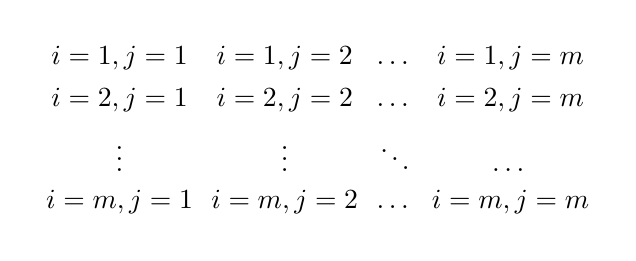
\begin{tikzpicture}
\matrix[matrix of nodes]{
$i=1,j=1$ & $i=1,j=2$ & $\dots$ & $i=1,j=m$ \\    $i=2,j=1$ & $i=2,j=2$ & $\dots$ & $i=2,j=m$ \\    $\vdots$ & $\vdots$ & $\ddots$ & $\dots$ \\ $i=m,j=1$ & $i=m,j=2$ & $\dots$ & $i=m,j=m$ \\% <- Without this %, there would be a trailing "1" in the copied text
};
\end{tikzpicture}

and observing that $\forall \, i=1,2,\dots m$, we're doing $m$ computations for $j$ and needing to fetch $m$ values for each $\lambda_j$, $y_j$, $X^{(j)}$, and so on.

Consider this computation: for a given, single $i\in \lbrace 1,2,\dots m\rbrace$, define 
\begin{equation}
f_{1i}(\lambda) := \frac{1}{2} \sum_{j=1}^m \lambda_j y^{(j)} K(X^{(i)},X^{(j)})
\end{equation}
For this step, we'll only need to do $m$ fetches for the $\lambda_j,y^{(j)},X^{(j)}$ values, and $X^{(i)}$ value will be fetched once.  As this is a summation over a potentially large vector ($m$ can be big), this looks like a good case/candidate for the usage of parallel \emph{reduce} algorithm.  The work complexity of parallel reduce is $O(\log{m})$ \cite{CS344}\footnote{\href{https://youtu.be/tSgVVVTe5KQ}{Step Complexity of Parallel Reduce - Intro to Parallel Programming, Udacity}}.  Theano has an implementation of reduce in \verb|theano.reduce|.

Once all $m$ $f_{1i}$'s are obtained, for $i=1,2,\dots m$, then parallel reduce can be used again (especially if $m$ is large!).  Also, empirically, I found that using \verb|theano.reduce| again helped to circumvent the problem of the maximum recursion limit for Python \footnote{\href{https://github.com/Theano/Theano/issues/689}{max recusion limit \#689}}, which is inherent with Python (cf. \verb|import sys  sys.getrecursionlimit()|).  In practice, above about 10000 recursions, the Python script fails with run-time errors.

Nevertheless, in this second (parallel) reduce step, we are doing
\[
f_1 = \sum_{i=1}^m \lambda_i y^{(i)} f_{1i}(\lambda)
\]
with $m$ fetches of values for $\lambda_i, y^{(i)}$.  The work complexity here for this reduce step is again $O(\log(m))$

Thus, we are doing, for 2 (parallel) reduces, $2m$ fetches (or reads), for each $\lambda_i$ or $y^{(i)}$ or $X^{(i)}$.

The total work complexity is $O(2\log(m))$.  

Likewise, for the computation of the intercept $b$ in Eqn. \ref{Eq:bintercept}, after minimizing $W(\lambda)$ by varying $\lambda$, I also employed parallel reduce via \verb|theano.reduce| (but only once for the single sum) and for the prediction step for $\widehat{y}$ in Eq. \ref{Eq:predictyhat}

\subsection{Code (theano/Python script), jupyter notebook accompanying code}\label{SubSec:Code}

SVM is implemented as described above, in particular Eqns. \ref{Eq:DualFormulationW}, \ref{Eq:ProjectionOpsAlgo}, in the Python class \verb|SVM_parallel|.  The default kernel function $K:\mathbb{R}^d\times \mathbb{R}^d \to \mathbb{R}^d$ is the radial basis function, which takes the form of a gaussian, is first implemented and I can implement other kernel functions easily, as a Python function object and Python class member, in the future.

Take note that for the (currently) implemented radial basis function, Python function (object) \verb|rbf| in \verb|SVM.py| of \href{https://github.com/ernestyalumni/MLgrabbag/blob/master/ML/SVM.py}{github:ernestyalumni/MLgrabbag/ML}, what's formulated is this:
\begin{equation}\label{Eq:rbf}
K(X^{(i)}, X^{(j)}) = \exp{ \left( - \frac{ \| X^{(i)} - X^{(j)} \|^2}{ 2\sigma^2 }  \right) } 
\end{equation}
with $K: \mathbb{R}^d \times \mathbb{R}^d \to \mathbb{R}$.

Take a look at the $\sigma \in \mathbb{R}$ parameter in Eq. \ref{Eq:rbf}.  $\sigma$ is analogous to the variance of a Gaussian (normal) distribution.  For other implementations, notably \verb|libsvm| and sci-kit learn, they use this form of the radial basis function:
\[
K(X^{(i)}, X^{(j)}) = \exp{ \left( - \gamma  \| X^{(i)} - X^{(j)} \|^2  \right) } 
\]
So $\gamma$ parameter here is equivalent to $\sigma$:
\[
\gamma = \frac{1}{2\sigma^2}
\]
While this redefinition makes no change to the formulation above, this is something to note when when using \verb|libsvm|, sci-kit learn, or \verb|SVM.py| here when manually inputting the parameters to train models.  


The theano/Python code follows directly from Eqns. \ref{Eq:DualFormulationW}, \ref{Eq:ProjectionOpsAlgo} and is in the \verb|/ML| subfolder of the github repository \verb|MLgrabbag| \footnote{\href{https://github.com/ernestyalumni/MLgrabbag/tree/master/ML}{github:ernestyalumni/MLgrabbag}}, in \verb|SVM.py|.  Wherever a summation is seen in the mathematical formulation, \verb|theano.reduce| is used.  

In the \verb|SVM_parallel| Python class method \verb|build_W|, I code a \verb|theano.reduce| inside a \verb|theano.reduce| and show it's possible to be done.  This represents, both formally and the parallel reduction on the GPU, the double summation that we sought to compute in \ref{Eq:DualFormulationW} for $W(\lambda)$.

The jupyter notebook \verb|SVM_theano.ipynb| in the same github repository steps through how I developed and used \verb|SVM_parallel|, training it on a number of sample datasets.  Because of the interactivity of jupyter notebook, I invite others to explore and play with the notebook if further clarification on \verb|SVM_parallel|, or how to use it, is needed \footnote{\href{https://github.com/ernestyalumni/MLgrabbag/blob/master/SVM_theano.ipynb}{github:ernestyalumni/MLgrabbag SVM theano.ipynb}}

\section{Immediate Results from training on sample datasets} \label{SubSec:ResultsSampleDatasets}

\subsection{Real-World Examples}

I trained a SVM on 2 of the real-world data sets provided by Hsu, Chang, and Lin \cite{HCL}, one for astroparticles and another for vehicles, using, for hardware, a NVIDIA GeForce GTX 980 Ti.  Checking the computational graph generated by theano (using \verb|theano.function.maker.fgraph.toposort()|), \verb|nvidia-smi -l 2| (monitoring real-time GPU usage), and the (usual, in Utilities) CPU resources System Monitor.

I will copy the results from Hsu, Chang, and Lin \cite{HCL} for comparison.  The accuracy measure is determined from the given \emph{test} data, \emph{not} on the training data (which is part of good machine learning and scientific practice).  

%\begin{table}
\begin{tabular}{l*{6}{c}r}
Applications & \# training data & \# testing data & \# features & \# classes \\
  \hline
Astroparticle\footnote{Courtesy of Jan Conrad from Uppsala University, Sweden} & 3089 & 4000 & 4 & 2 \\
Vehicle\footnote{Courtesy of a(n anonymous) user from Germany} & 1243 & 41 & 21 & 2  \\
  \end{tabular}  \\
%\caption{Table 1: Sample Dataset Problem characteristics and accuracy performance \cite{HCL}}

\begin{tabular}{l*{2}{c}r}
Applications & $C=$ & $\gamma=$ & Accuracy by \verb|libsvm|  \\
\hline
Astroparticle &  2.0 & 2.0 & 96.9\% \\
Vehicle &  128.0    & 0.125 & 87.8\%
  \end{tabular}

Table 1: Sample Dataset Problem characteristics and accuracy performance \cite{HCL}. \\
%\end{table}


%\begin{table}
\begin{tabular}{l*{5}{c}r}
Applications & $C=$ & $\sigma=$ & $\alpha=$ & \# iterations  \\
\hline
Astroparticle & 2.0 & 0.30 & 0.001 & 15  \\
Vehicle      & 128.0 & 2.0 & 0.001 & 20   \\
\end{tabular}  \\
%\end{table}
\begin{tabular}{l*{1}{c}r}
Applications & Time to train (on GTX 980Ti) & Accuracy by \verb|SVM_parallel|   \\
\hline
Astroparticle &  1h 7min 18s & 96.1\% \\
Vehicle & 14min 54s  & 95.1\% \\
\end{tabular} \\

Table 2: Results of training on Sample Datasets with \verb|SVM_parallel|  \\

The very last result testing on the test data for vehicles is promising for \verb|SVM_parallel|.  At this point, I would invite others to suggest sample and real-world datasets to train and test on, using \verb|SVM_parallel|, as I also try to find other datasets, and add onto the jupyter notebook \href{https://github.com/ernestyalumni/MLgrabbag/blob/master/SVM_theano.ipynb}{SVM theano.ipynb on github}.  It'd be interesting to vary the \emph{number of training examples}, to find a dataset with more than 10000 ($m>10000$) examples and see how \verb|SVM_parallel| can scale with large data sets (indeed, for $m>10000$, the SVM would have $m>10000$ support vectors in the model), and vary the \emph{number of features} (whether SVM does better with large or small number of features, relative to $m$).

\section{Conclusions/Summary/Dictionary between Math and Code}\label{Sec:ConclusionsSummary}

I had reviewed the motivation and derivations for SVM.

What's novel is that, given the GPU(s), I implemented \emph{constrained gradient descent} or \emph{projected gradient descent}, for training models, instead of Quadratic Programming, that computes a quadratic form (to tackle the double summation in the dual formulation), through SMO, as used before (e.g. \verb|libsvm|, sci-kit learn).  Its (\emph{constrained gradient descent} or its implementation here \verb|SVM_parallel|) work complexity is $O(2\log{m})$, as opposed to $O(m^2)$.  This was achieved by using theano's reduce, inside a reduce.  

Its (i.e. \verb|SVM_parallel|) promising to be scalable to large datasets ($m>10000$).  I seek to find large datasets to train and test on and are appropriate for binary classification, and invite others to make suggestions or play with the code and jupyter notebook itself.

I'll provide a 1-to-1 dictionary here between the mathematical formulation and the Python code.  As a note on software engineering, object-oriented programming (OOP) and how to code classes, I had sought to identify (make isomorphisms) and design Python classes and function objects with 1-to-1 correspondence to the mathematical formulation.  The hope is that it would allow other developers to rapidly make progress in improving upon the code or to rapidly understand its usage and apply it as they'd like to see fit.  

\[
\begin{aligned}
  \begin{gathered}
    \text{ we seek to minimize } \\
    W(\lambda) = - \sum_{i=1}^m \lambda_i + \frac{1}{2} \sum_{i,j=1}^m \lambda_i \lambda_j y^{(i)} y^{(j)} K(X^{(i)},X^{(j)}) 
  \end{gathered} \quad & \quad   \verb|SVM_parallel.build_W| \\
  \text{  by iterating $t=0,1,\dots $, as such: } \qquad \, & \quad \\
  \qquad \, \verb|SVM_parallel.train_mode_full(max_iters=250)|  & \quad \\
  \begin{aligned}
    & \lambda_i'(t+1):=\lambda_i(t) - \alpha \text{grad}{ W(\lambda) } \\ 
    & \lambda''_i(t+1):= \mathbf{P}_{\sum_{i=1}^m \lambda_i y^{(i)} = 0 }( \lambda_i'(t+1)) \\ 
    & \lambda_i(t+1) := \Pi_{0\leq \lambda_i \leq C}(\lambda_i''(t+1))
  \end{aligned} \quad \, &
  \quad \, \verb|SVM_parallel.build_update|  
  \end{aligned}
\]
where
\[
\begin{gathered}
\mathbf{P}_{\sum_{i=1}^m \lambda_i y^{(i)} = 0 }( \lambda_i'(t+1)) = \lambda_i'(t+1) - \frac{ \sum_{i=1}^m y^{(i)}\lambda_i'(t+1) }{ \sum_{i=1}^m (y^{(i)})^2 } y^{(i)} \\ 
\Longleftrightarrow \\
\verb|updatelambda_mult=updatelambda_mult-T.dot(y,updatelambda_mult)/T.dot(y,y)*y| \\
\text{ in } \verb|SVM.build_update|
\end{gathered}
\]

\[
\begin{gathered}
  \begin{aligned}
  & \Pi_{0\leq \lambda_i \leq C}(\lambda_i''(t+1)) = \begin{cases} C & \text{ if } \lambda_i''(t+1) > C \\
    \lambda_i''(t+1) & \text{ if } 0 \leq \lambda_i''(t+1) \leq C \\
    0 & \text{ if } \lambda_i'(t+1) <0 \end{cases}
  \end{aligned}  \\ 
  \Longleftrightarrow \\
  \begin{aligned}
    & \verb|updatelambda_mult=T.switch(T.lt(C,updatelambda_mult),C,updatelambda_mult)| \\
    & \text{ in } \verb|SVM.build_update| \\ 
    & \verb|updatelambda_mult=T.switch(T.lt(updatelambda_mult,lower_bound),| \\
    & \verb|lower_bound,updatelambda_mult)| \\
    & \text{ in } \verb|SVM.build_update| 
      \end{aligned}
  \end{gathered}
  \]

Finally, to tie it back into my original motivation, now that SVM is natively implemented in theano, it would be interesting to try to develop (and of course find appropriate datasets to train and test on) a DNN that will have as its ``outer'' or last layer to be a SVM.  Since SVM is now part of the theano computational graph, optimization (the so-called ``backpropagation'' step) will be done automatically and simply with theano's \verb|grad|, on all the parameters or ``weights'' of the entire model.  





\begin{thebibliography}{9}

\bibitem{CS344}
John Owens.  David Luebki.  \emph{Intro to Parallel Programming}.  \emph{CS344}.  \textbf{\href{https://www.udacity.com/}{Udacity}}  
  



\bibitem{Nowa2008}
Thomas Nowak.  ``Implementation and Evaluation of a Support Vector Machine on an 8-bit Microcontroller.''  Univ.Ass. Dipl.-Ing. Dr.techn. Wilfried Elmenreich Institut f\"{u}r Technische Informatik Fakult\"{a}t f\"{u}r Informatik Technische Universit\"{a}t Wien.  Juli 2008.  \url{https://www.lri.fr/~nowak/misc/bakk.pdf}





\bibitem{ChZa2013}
Edwin K. P. Chong and Stanislaw H. Zak.  \textbf{An Introduction to Optimization}.  4th Edition.  Wiley.  (January 14, 2013).  ISBN-13: 978-1118279014
  


\bibitem{Bish2007}
Christopher M. Bishop.  \textbf{Pattern Recognition and Machine Learning} (Information Science and Statistics).  Springer (October 1, 2007).  ISBN-13: 978-0387310732


\bibitem{CFZ2009}
Bertrand Clarke, Ernest Fokoue, Hao Helen Zhang.   \textbf{Principles and Theory for Data Mining and Machine Learning} (Springer Series in Statistics)  Springer; 2009 edition (July 30, 2009).  ISBN-13: 978-0387981345
 

\bibitem{Ngu2007}
Hubert Nguyen. \textbf{GPU Gems 3}.  Addison-Wesley Professional (August 12, 2007).  ISBN-13: 978-0321515261.  Also made available in its entirety online at \url{https://developer.nvidia.com/gpugems/GPUGems3/gpugems3_pref01.html}

\bibitem{Pedr2011}
  Scikit-learn: Machine Learning in Python, Pedregosa \emph{et al.}, \textbf{JMLR 12}, pp. 2825-2830, 2011.

\bibitem{ChLi2011}
  C.-C. Chang and C.-J. Lin. \emph{LIBSVM : a library for support vector machines}. \textbf{ACM Transactions on Intelligent Systems and Technology}, 2:27:1--27:27, 2011. 

\bibitem{Pla1998}
  J. Platt. \emph{Fast training of support vector machines using sequential minimal optimization}. In A. Smola B. Schölkopf, C. Burges, editor, \textbf{Advances in Kernel Methods: Support Vector Learning}. MIT Press, Cambridge, MA, 1998.

\bibitem{HCL}
Chih-Wei Hsu, Chih-Chung Chang, and Chih-Jen Lin.  \emph{A Practical Guide to Support Vector Classification}.  \url{http://www.ee.columbia.edu/~sfchang/course/spr/papers/svm-practical-guide.pdf}

  
\end{thebibliography}



\end{document}
